\chapter{Diskussion af resultater}

I dette kapitel vil der blive diskuteret relevante dele af de opnåede resultater og deres betydning for bachelorprojektet, samt hvilke muligheder og begrænsninger der er ved anvendelse af SRM. 

\section{Konstant strøm}
Ud fra de forløbende tests kom strømmen til at ændre sig. Ønsket var en konstant strøm på 283 $\mu A$. Problemet ved ikke at have en fast strøm gør, at det ikke bliver valide BI signaler, da denne faste strøm bruges til at udregne impedansen af BI signalet til en senere visning. Strømmen faldt til 104 $\mu A$, da elektroderne blev påmonteret måleobjektet, hvilket ikke stemmer overens med den beregnede 283 $\mu A$. Da MyoWare Muscle Sensor blev tilføjet steg strømmen igen til 283 $\mu A$. Det kan skyldes det at MyoWare Muscle Sensor bruger en reference elektrode som har fælles stel med BI måleren. Dette er ikke med i designet og derfor ikke tage høje for dette. Det kan være en mulig tilføjelse til BI måleren, da referance elektrode bliver brugt hvor man ønsker at måle BI signaler simultant med EMG signaler\cite{Nahrstaedt2012a}. 

\section{AA filter}
BI signalet afhænger af at AA filteret er korrekt bygget og fungere efter hensigten. Ellers vil den efterfølgende signalbehandling og visning af signalet være ubrugeligt. Testene viser at AA filter fungerer efter hensigten ved at det bliver dæmpet ned til 95 dB ved 250 kHz. 

\section{to målinger simultant}
Ved at kunne foretage simultane målinger med BI og EMG signal, er hele konceptet med at have disse to parametre. Dette ville gøre detektionen af et synk endnu mere valide,da der vil kunne konkluderes om det var et synk og ikke en anden bevægelse. 



\section{Elektrode placering}
Ved brug af de store EKG elektroder, var der ikke så stor fleksibilitet mht. placeringen af disse elektroder. Inspiration af placering af eletroderne blev fundet i flere artikler.\cite{Chester}
\cite{Schultheiss2013} Det at flytte rundt på elektroderne placering i forhold til hinaden ændre også BI signalet\cite{Yamamoto2000}.  



\section{Digital signal behandling}
Da signalerne er samlet ved en forholdsvis høj sampling rate på 500 kHz, giver det en stor mængde data. Med fordel kan denne store mængde være med til at det er muligt at signal behandlet BI signal i det digitale domæne.
dobbelt ensretter
filterer

\section{GUI - simultane signaler, kan se synk og der tælles synk}


\begin{figure}[H]
\centering
\begin{minipage}{.5\textwidth}
  \centering
  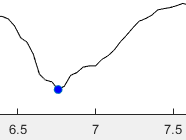
\includegraphics[width=.8\linewidth]{Figure/synkfraGUI}
  \captionof{figure}{Strømmen uden påsatte elektroder}
  \label{fig:integrationstestVCCSud}
\end{minipage}%
\begin{minipage}{.5\textwidth}
  \centering
  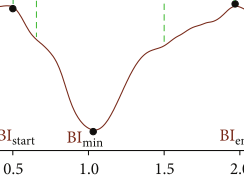
\includegraphics[width=.8\linewidth]{Figure/synkfraArtikel}
  \captionof{figure}{Strømmen med påsatte elektroder}
  \label{fig:integrationstestINA2udstrom}
\end{minipage}
\end{figure}


\begin{figure}[H]
\centering
{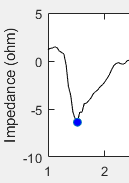
\includegraphics[width=4cm]
{Figure/synkfraGUI5ohm}}
\caption{Figuren viser designet af GUI til SRM.}
\label{Fig:designGUI}
\end{figure} 

\section{Relation til problemformulering}

\section{Resultat vi særlig stolte af}

